\chapter{Používané metody testování}
V této kapitole se pokusím popsat co nejvíce známých pohledů a způsobů na testování, aby bylo dále možné vybrat, aplikovat a navrhovat testovací systém s ohledem na dnešní metody a trendy v testování. Nejdříve popíšu úrovně testování, kterými by měl každý výrobek před uvedením na trh projít. Dále popíši způsoby  testování, kterými může testování proběhnout. V poslední kapitole jsou popsány další nezařazené možné pohledy a přístupy k testování.

\section{Úrovně testování}
Testování výrobků před uvedením na trh prochází několika stupni testování. Některé stupně jsou při vývoji používány bez toho, aby si to vývojáři uvědomili a jiné důležité stupně testování jsou zase často opomíjeny. Mnou rozebíraný model má celkem 5 stupňů testování. Jednotlivé stupně dále popíši a rozeberu jejich přínos a možnosti použití v mém testovacím systému.

\begin{figure}[h]
  \centering
  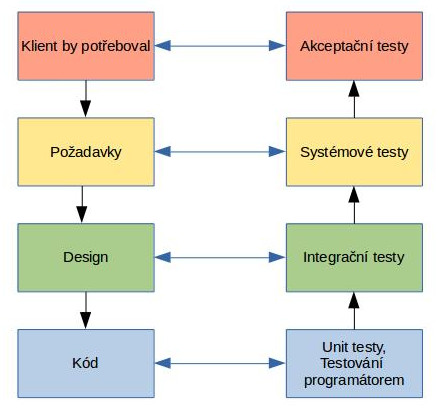
\includegraphics[width=.6\LW]{test_phase}
  \caption{Schéma testovacího modelu}
  \label{fig:test_phase}
\end{figure}

\subsection{Testování programátorem (Developer testing)}
První a úplně nezbytnou fázi testování by měli provádět programátoři. Programátor by si měl zkontrolovat jestli je možné firmware přeložit a dále jestli jeho nová či opravená funkcionalita funguje správně. V další fázi testování by měl zkontrolovat kód jiný programátor, který kód nepsal. Tuto fázi většinou provádí správce projektu při zařazování nové či upravené funkce do hlavní větve repozitáře projektu. Všechny chyby odchycené v této fázi testování ušetří spoustu času stráveném v dalších fázích testování.

Testování programátorem může vypadat jako samozřejmá věc, která by nemusela být ani uváděna. Bohužel opak je pravdou a i tato situace může nastat. V případě že je tato fáze vynechána je pravděpodobné že spousta chyb je odhaleno až ve fázi systémového testování, kdy zjišťování, reportování a oprava chyb stojí značnou režii.

\subsection{Testování jednotek (Unit testing)}
Úroveň testování jednotek obsahuje testování jednotlivých částí nebo modulů softwaru. Za jednotku neboli část lze považovat objekt s jednou jedinou funkcionalitou, a to například třídu, objekt, program či softwarový modul. Tato úroveň testování testuje správnost zdrojového kódu a ne funkci programu jako celku. Velmi známým příkladem jsou JUnit testy v javě, kde ke každé třídě a metodě je vytvářena testovací třída či metoda.

Unit testy je výhodné použít při tvorbě nového projektu, jelikož s unit testy je potřeba počítat již při návrhu zdrojového kódu a při návrhu kódu zároveň testy vytvářet. Dopisování testů do již existujícího projektu by stálo neúměrnou námahu a mnoho úprav kódu pro přizpůsobování samotného programu pro unit testování.

Zdrojový kód pro výrobky testované navrhovaným testovacím systémem je vyvíjen již 10 let a zároveň na těchto zdrojových kódech jsou stavěny i nové výrobky. Navíc přes devadesát procent firmwaru používá opensource řešení. Díky těmto dvěma skutečnostem je v nynější situaci nereálné přidat unit testování do navrhovaného testovacího schématu.

\subsection{Integrační testování (Integration testing)}
Po předchozích dvou úrovních testování, jenž jsou prováděny programátory, přichází fáze, kdy se hotový výrobek dostává do ruky testerům. Testeři většinou provádí dvě úrovně testování, integrační testování a systémové testování. Někdy jsou tyto dvě fáze spojovány do jedné a nazývají se systémově integrační testování. Obě úrovně budou dále detailněji popsány.

\begin{figure}[h]
  \centering
  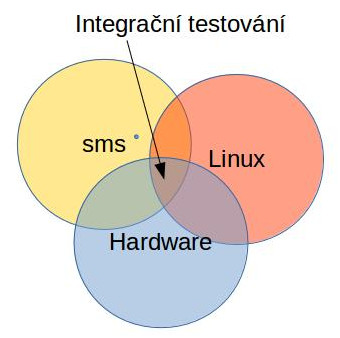
\includegraphics[width=.4\LW]{test_integration}
  \caption{Grafické znázornění integračního testování}
  \label{fig:test_integration}
\end{figure}

Pomocí integračního testování testujeme integraci jednotlivých komponent mezi ostatní komponenty, dále také integraci jednotlivých komponent do operačního systému, či na konkrétní hardware. Jako příklad mohu uvést testování integrace programu odesílání sms zpráv na operačním systému Linux, běžícím na hardwaru konkrétního routeru. Příklad znázorňuje, že není testováno pouze odesílání sms zpráv, ale komponenta v závislosti na operačním systému a hardwaru. Jednotlivé komponenty mohou být například subsystémy, databázové implementace, infrastruktura, rozhraní a systémové konfigurace. Integrační testování lze z testování vypustit, jelikož chyby nalezené v této fázi by byly odhaleny ve fázi systémového testování, nýbrž za cenu vyšší časové náročnosti.

Integrační testy navrhují testeři na základě čtyř základních skutečností a to softwárový a systémový design výrobku, architekturu firmwaru, pracovního postupu s danou komponentou a možnými případy použití. Na základě těchto čtyř skutečností tester navrhne testovací případy a postupy. Podle těchto postupů jsou jednotlivé komponenty dále testovány manuálně testery či automaticky automatem.

Testovací automat bude v prvním kroku testovat integračními testy všechny základní komponenty routeru, jako například posílání SMS zpráv, či SMPT klient vůči operačnímu systému Linux či uCLinux běžícím na každém z 50 různých výrobků podporujících testovanou funkcionalitu. Zde je nejlépe vidět přínos testovacího automatu. Ve skutečnosti by tester měl provést test integrace všech funkcionalit na všech padesáti odlišných výrobcích, což je časově značně náročné. Zatímco automat tento test může provést každý den na všech výrobcích paralelně během chvilky. Tímto testováním je ověřena integrace daného programu na všech výrobcích a neunikne žádná chyba způsobená chybou v firmwaru, či chybou některé ze součástí routeru, čímž může být například odlišná implementace odesílání sms v bezdrátovém modulu.

\subsection{SIT - Systémové testování (System testing)}
Systémové testování je poslední fází testování probíhající ve společnosti vyvíjecí daný produkt. Ve fázi systémového testování se testuje výrobek jako celek z pohledu zákazníka. Jsou navrhnuty jednotlivé testovací případy, které mohou nastat v praxi, a dle těchto případů jsou výrobky testovány. Příklad takového testovacího scénáře může být testovaný router do kterého je přes Ethernet připojena IP kamera a přes sériové rozhraní teplotní senzor. Data z těchto zařízení jsou přes OpenVPN tunel sestavený přes mobilní spojení posílána na vzdálený server.

\begin{figure}[h]
  \centering
  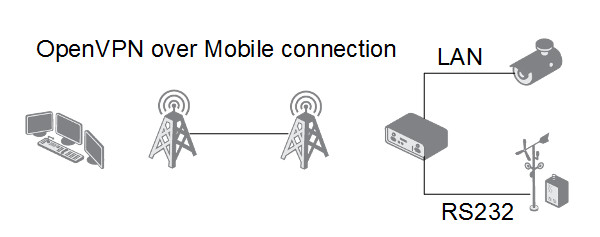
\includegraphics[width=.8\LW]{system_test_example}
  \caption{Příklad systémového testování}
  \label{fig:system_test_example}
\end{figure}

Systémové testy mohou obsahovat funkční i nefunkční testy, které jsou dále popsané v sekci věnované těmto typům testování. Dále je možné testovat kvalitu či rychlost přenosu dat, které mohou být prováděny na výrobcích ve standartním, ale i ve stiženém prostředí, například v klimatické komoře nebo v okolí EMC vyzařovaní. Na systémové testování je také možné pohlížet jako na testování bílé či černé skříňky. Oba způsoby jsou také dále popsány v kapitole věnující se dalším typům testování.

V navrhovaném případě testování bude systémové testování prováděno ve stejném kroku a pomocí stejných nástrojů jako integrační testování, čili tento model se blíží dříve zmíněné možnosti spojení systémových a integračních testů. V navrhovaném případě testování lze někdy určit hranici mezi systémovými a integračními testy a někdy je toto rozdělení obtížné určit. Většina systémových testů obdobně jako integrační testy bude možné provádět automaticky pomocí testovacího automatu. Jiné systémové testy, jako například testy v klimatické komoře, budou muset být dále z kapacitních důvodů prováděny manuálně, jelikož všech padesát výrobků se do klimatické komory nevejde. Naopak tyto testy nezávisí na změně firmwaru, čili ve většině případech stačí pouze jedno provedení klimatických testů při vyvinutí nového hardwaru výrobku a ne při každé změně firmwaru.

\subsection{UAT - Akceptační testování (Acceptance testing)}
Poslední úrovní testování je akceptační testování. Akceptační testování již není prováděno testery ve firmě, kde je výrobek vyvíjen. Testování je prováděno u cílového zákazníka na konkrétní aplikaci výrobku. Případné chyby či nesrovnalosti od požadované funkcionality jsou reportovány zpět a bývá očekávána rychlá reakce na opravu těchto chyb. Snaha testovacího systému samozřejmě bude odhalit všechny případné chyby před touto úrovní, tedy před dodáním výrobku zákazníkovi. Jelikož se tato fáze provádí až u koncového zákazníka, práce se touto fází dále nebude zabývat.

\section{Testovací procesy}
Fáze systémového a integračního testování lze provádět pomocí třech různých přístupů k testování. Všechny tři přístupy se od sebe liší hlavně v délce a složitosti návrhu testování a v délce samotného provádění testů. V neposlední řadě se liší jejich pokrytí testovacích případů a tím i kvalita testování. Podle složitosti návrhu testů by bylo možné popisované přístupy testování seřadit sestupně na testování založené na modelech, automatizované testování a poslední manuální testování. Rychlostí a efektivitou provádění testů jsou tyto způsoby seřazeny přesně opačně. Cílem této práce je automatizovat a tím zkrátit provádění testů a zároveň rozšířit možností testování. Z cíle práce tedy vyplývá, že se budu snažit pokusit o přechod z nynějšího manuálního testování na automatizované testování a v nejlepším případě na testování založené na modelech.

\subsection{Manuální testování}
Prvním přístupem provádění testů je manuální testování. Manuální testování je možné rozdělit do dvou nezávislých kroků. Prvním krokem každého manuálního testování je vytvoření testovacího plánu. Testovací plán obsahuje informace o tom, co by mělo být na výrobku testováno, jak by měl být výrobek testován a nakonec jak často by měl být výrobek testován. Dle tohoto plánů navrhuje testovací technik testovací scénáře a jejich jednotlivé testovací procedury. Navrhování testovacích procedur se provádí pokaždé při změně nebo přidání funkcionality výrobku. Návrh provádí testovací technik s požadovanými znalostmi o testovaném výrobku.

\begin{figure}[h]
  \centering
  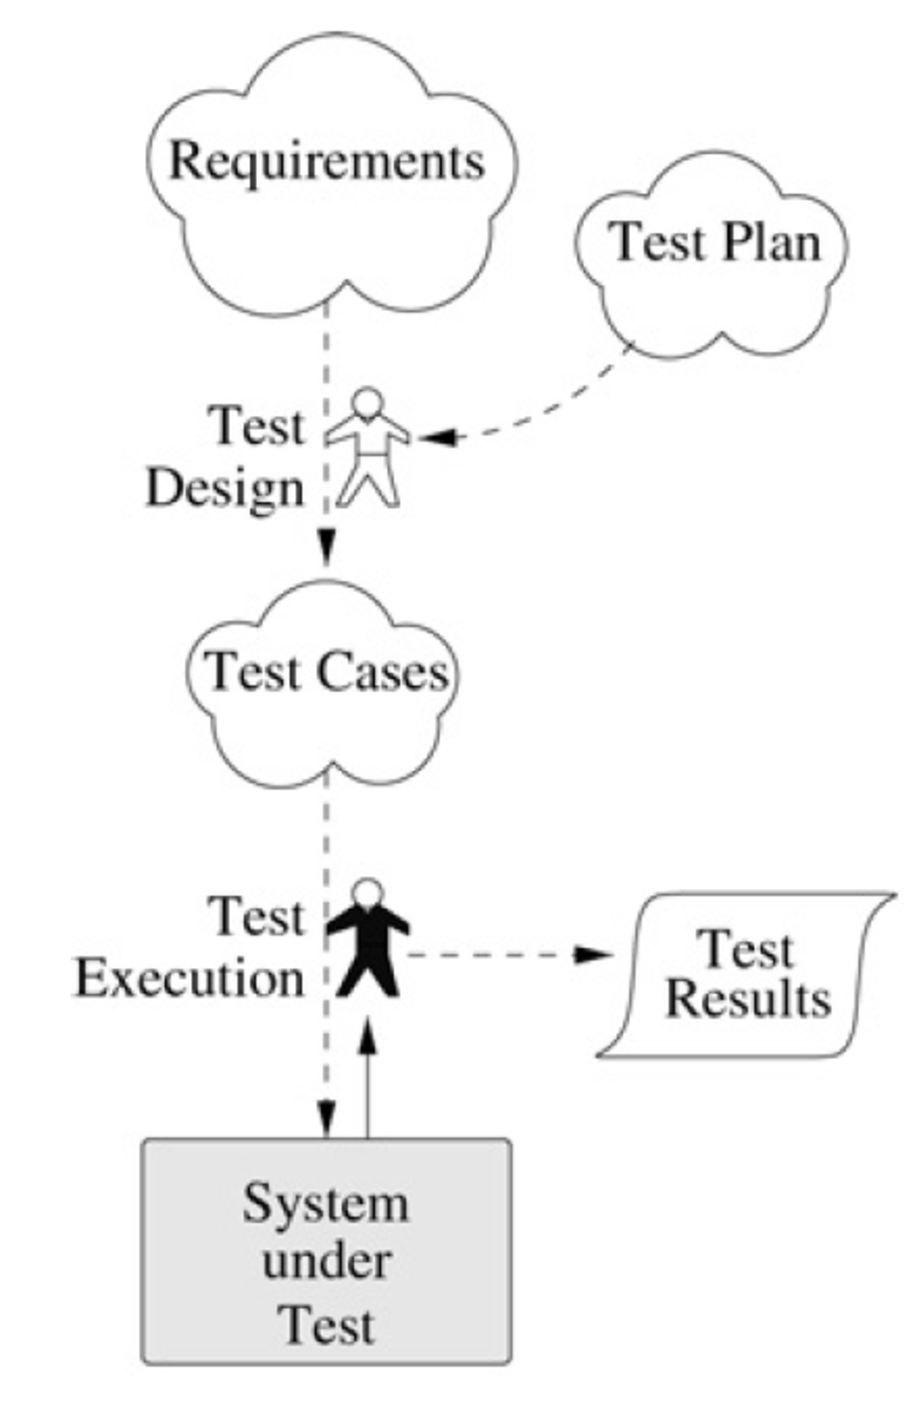
\includegraphics[width=.4\LW]{test_manual}
  \caption{Schéma manuálního testování}
  \label{fig:test_manual}
\end{figure}

Druhou fází manuálního testování je samotné provádění testů. Testy se provádějí manuálně přímo na testovaném objektu podle předepsaných testovacích procedur. Provádění testů je opakováno při každé změně ve firmwaru výrobku a dle jeho komplexnosti bývá i velice časově náročný. Z toho důvodu bývají některé testy vypouštěny, ale na úkor kvality testování celého výrobku. Samotné testování je práce manuální dle předepsaných pokynů a také velmi často se opakující, z toho plyne, že tuto práci může vykonávat tester bez znalostí návrhu testování samotných výrobků a jejich technologií. Dále se tento proces přímo nabízí k nějakému zlepšení jakoukoliv automatizací.

Ve společnosti, kde bude testovací systém nasazován, se nyní všechny testy provádějí manuálně dle předepsaných testovacích procedur. Jak už bylo v úvodu zmíněno, při rychle rostoucím počtu výrobků a jejich funkcionalit je nadále tento systém testování neudržitelný. Provádění integračních a systémových testů se budu snažit přesunout do jednoho ze sofistikovanějších způsobů testování. Dále pro specifické testy jako například EMC testy a klimatické testy v teplotní komoře nebude z kapacitních důvodů možné plně automatizovat a bude možné navrhnout moduly pro zjednodušené manuální testování.

Mohou nastávat i případy manuálního testování, kdy nejsou vytvořeny testovací plány a testovací procedury, kde je možné později doložit adekvátní výsledky testování. Další nevýhodou tohoto přístupu k testování je vynechání velkého množství testovacích případů, jelikož se jedná spíše o náhodné testování, proto tento postup není určitě doporučován.

\subsection{Automatizované testování}
Druhým a sofistikovanějším způsobem provádění testů je automatizované testování, někdy také nazývané testování založené na skriptech. Automatizované testování lze rozdělit do třech základních fází. První fáze vytvoření testovacího plánu je shodná s manuálním testováním.

\begin{figure}[h]
  \centering
  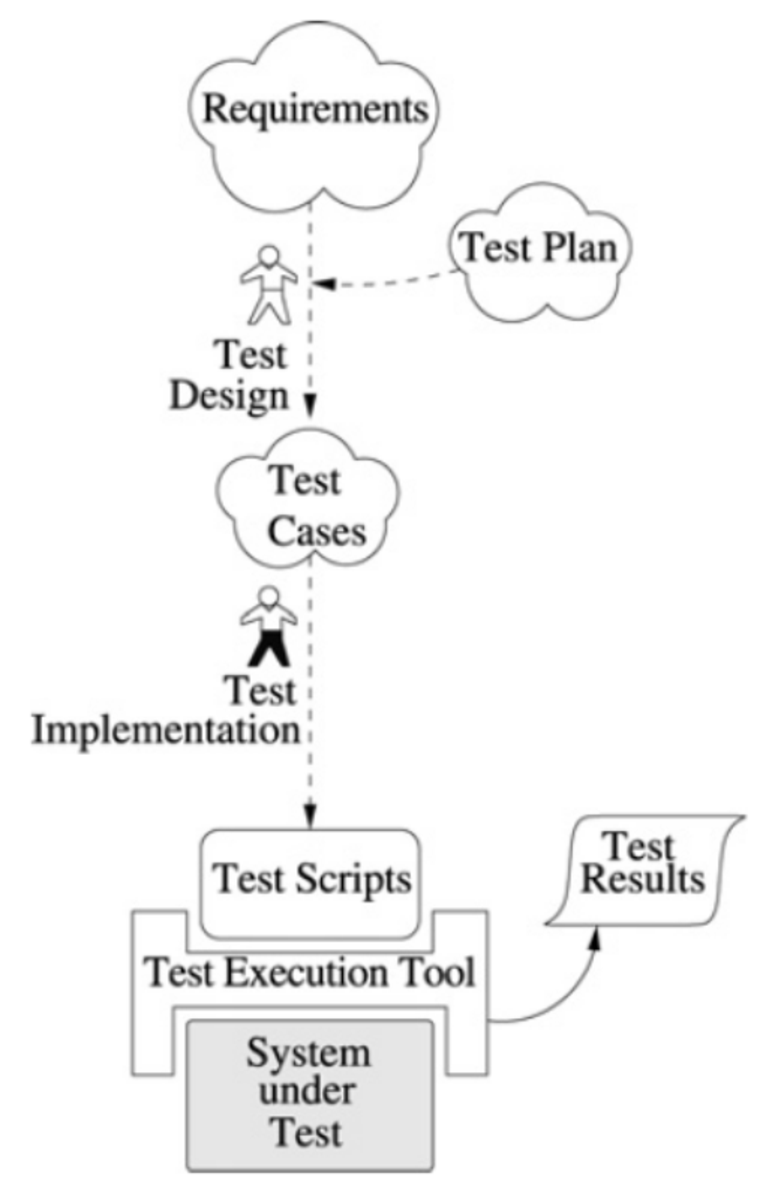
\includegraphics[width=.4\LW]{test_automat}
  \caption{Schéma automatického testování}
  \label{fig:test_automat}
\end{figure}

Druhou fází automatického testování je implementace testovacích procedur do spustitelných skriptů. Skriptovací testy mohou být napsány v nějakém standardním programovacím či skriptovacím jazyku nebo v jazyku přímo určenému k psaní testovacích skriptů. V našem systému bude k psaní testovacích skriptů použit skriptovací jazyk Bash a jednoduché programy napsané v programovací jazyk C. V automatizovaném přístupu testování nám přibyla další role programátora potřebného k implementaci testovacích procedur do spustitelných skriptů. Testovací skript je spustitelný skript nebo program, který provede jednu testovací proceduru. Testovací skript obvykle obsahuje inicializaci testovacího zařízení, uvedení testovacího zařízení do požadovaného kontextu, vytvoření vstupních testovacích hodnot, předání vstupních hodnot do testovaného zařízení, nahrání odpovědi od testovaného zařízení, nakonec porovnání odpovědi a očekávaného výstupu a vyhodnocení výsledku.

Třetí fází automatického testování je automatické spouštění testů. Testy jsou spouštěny automaticky pomocí nástroje pro spouštění testů. Nástroj provádí spouštění testů automaticky bez interakce s obsluhou. Nástroj navíc obsahuje možnost paralelizace testů nezávislých na nějakém zdroji. Zde je vidět veliká časová a tedy i finanční úspora oproti manuálnímu testování. Jestliže chceme provést nový test zařízení, spustíme pouze testovací nástroj a není potřeba manuálně testovat všechny funkcionality.

Naopak tento přístup přináší větší režii při změně funkcionality či přidání nového zařízení. Pokud je změněna testovací procedura či přímo funkcionalita výrobku, musí být předělány a přidány testovací skripty. Tato údržba může být v případech intenzivního vývoje stejně časově nákladná jako tvorba nových testovacích procedur pro danou funkcionalitu.

\subsection{Testování založené na modelech}
Nejsofistikovanějším řešením testování je testování založené na modelech, známé taky jako MBT (Model Base Testing). Zjednodušeně lze model tohoto systému popsat následovně. Tester vytvoří model testovaného zařízení, z tohoto modelu se automaticky vygenerují testovací skripty, které jsou spouštěny nad testovaným výrobkem. U tohoto testování odpadá spoustu času při návrhu a úpravách testovacích skriptů. Naproti tomu je velmi časově náročné navrhnutí samotného testovacího systému a modelu testovaného výrobku. Samozřejmě, že všechno není tak jednoduché, jak se na první pohled zdá a tak dále jsou detailně popsány všechny fáze tohoto způsobu testování. Jednotlivé fáze MBT jsou vývoj modelu testovaného zařízení, generování abstraktních testů z modelu, převedení abstraktních testů na spustitelné testy, spuštění testů na testovaném zařízení a analýza výsledků testů.

\begin{figure}[h]
  \centering
  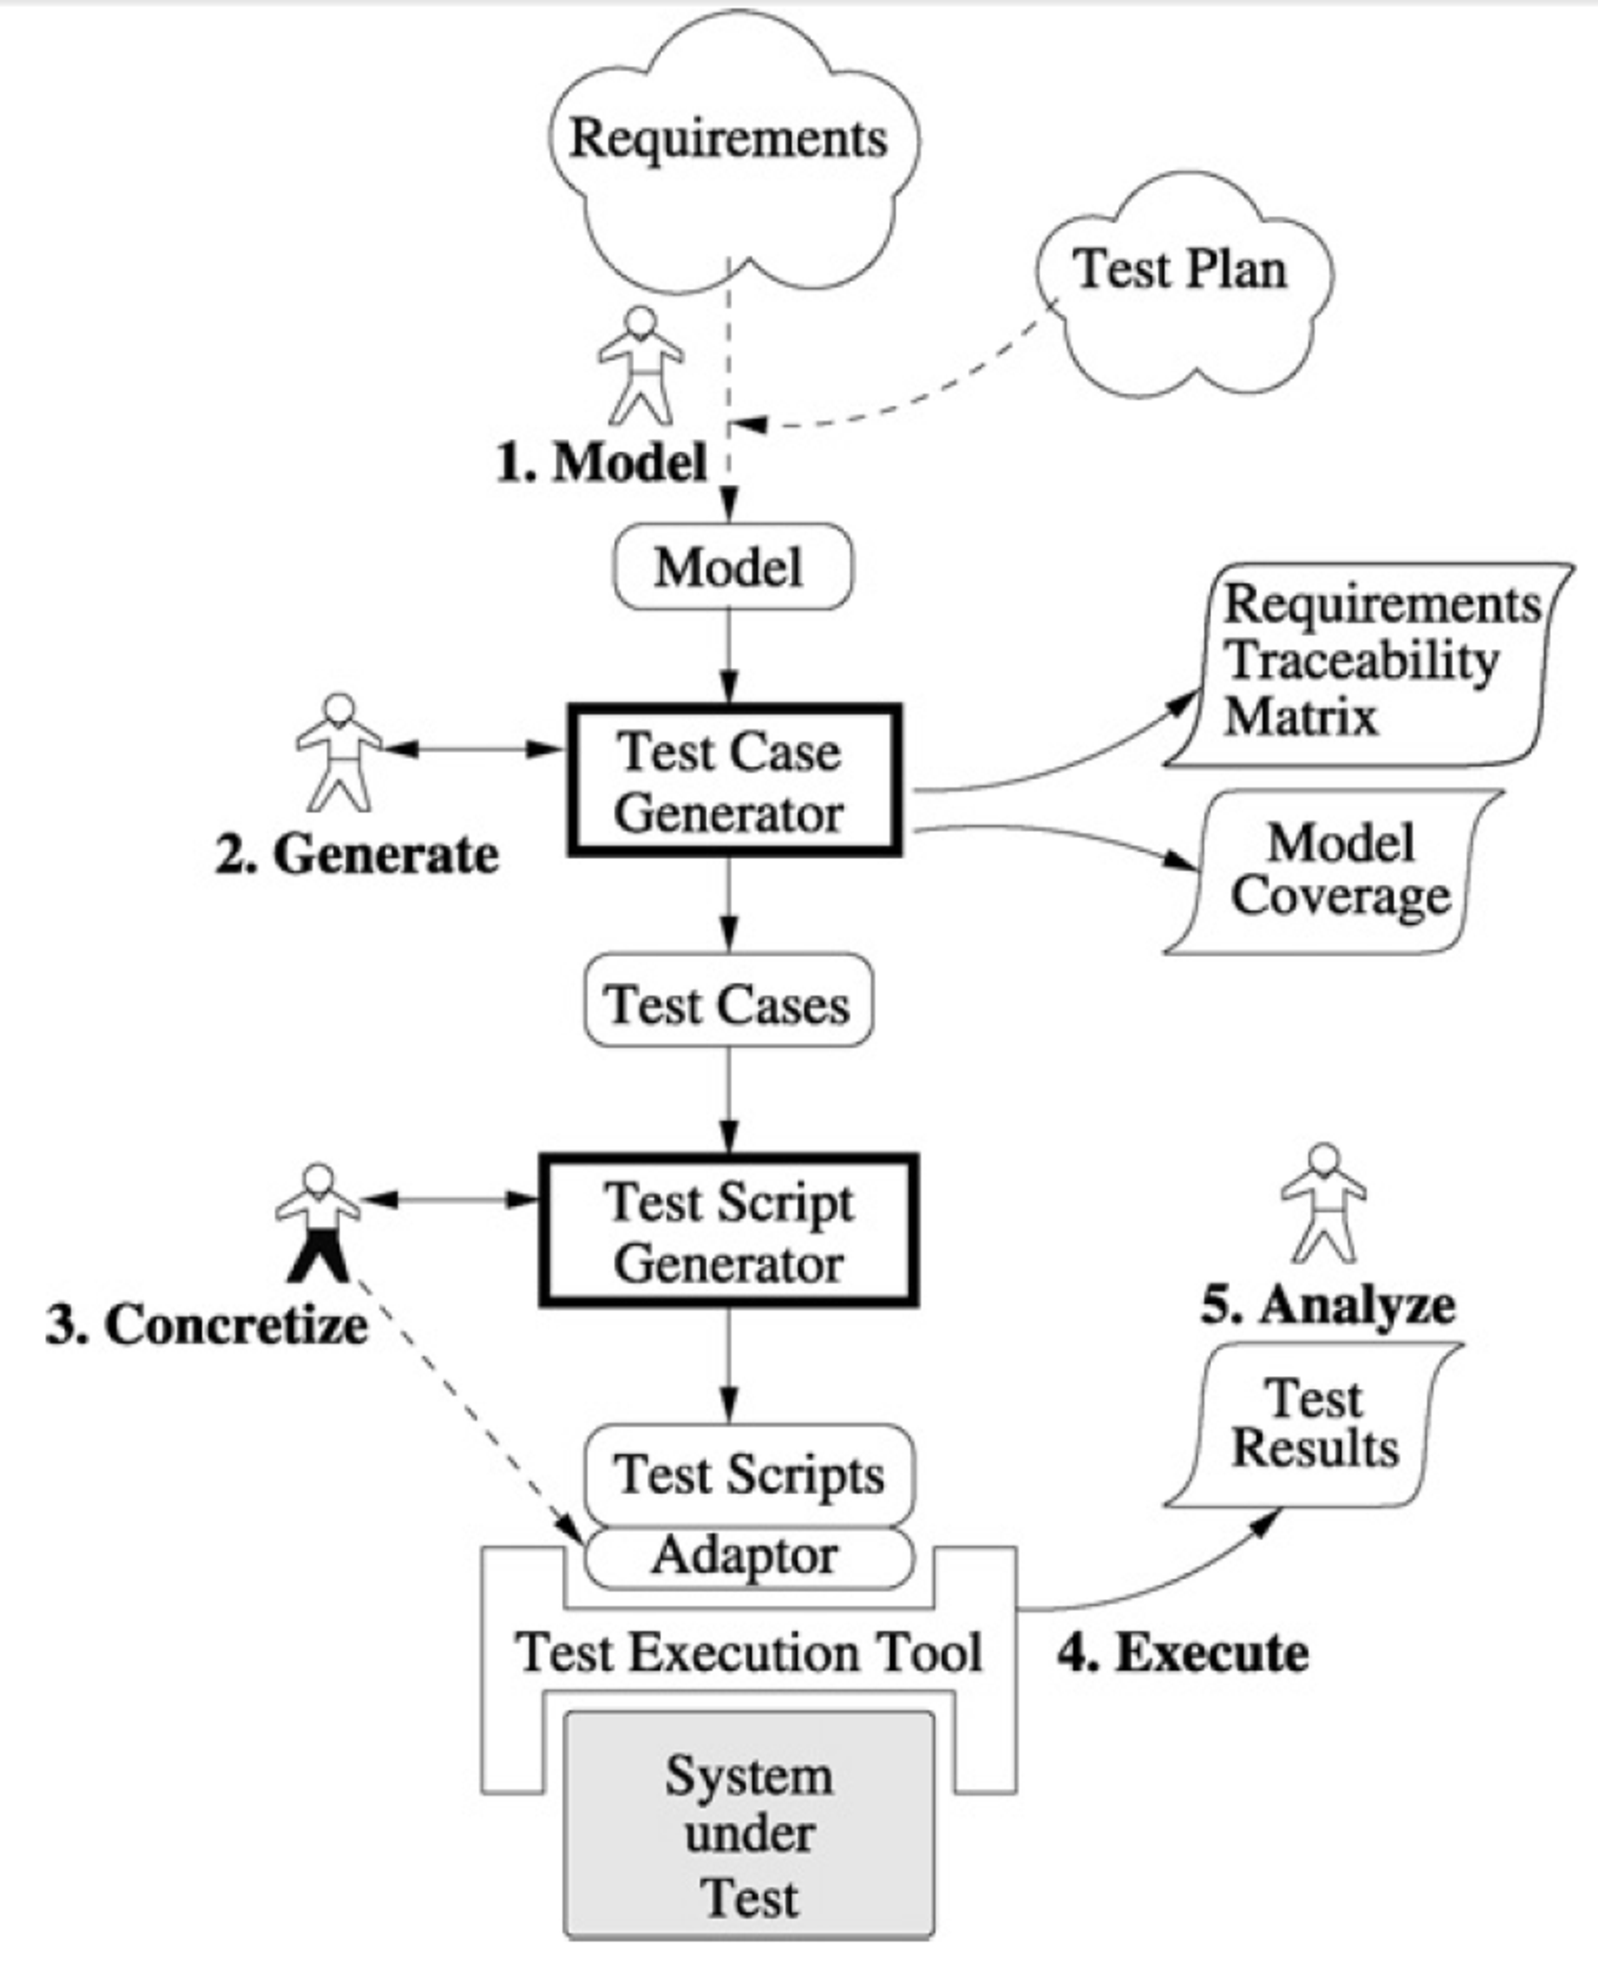
\includegraphics[width=.5\LW]{test_model}
  \caption{Schéma testování založeného na modelech}
  \label{fig:test_model}
\end{figure}

Prvním krokem testování založeném na modelech je tedy vytvoření abstraktního modelu testovaného zařízení. Model by měl být jednodušší nežli samotné zařízení a měl by se zaměřit na jeho klíčové vlastnosti.

Druhým krokem testování založeném na modelech je generování abstraktních testů z hotového modelu. Jelikož by ve většině případů bylo vygenerováno nekonečné množství testovacích případů, tak je potřeba určit nějaká testovací kritéria, aby bylo možné vygenerovat konečné množství testů. Tyto testy jsou sekvencí operací nad modelem. Používají zjednodušený pohled na testované zařízení a nejsou přímo spustitelné.

Třetí částí testování založeném na modelech je transformace abstraktních testů na spustitelné konkrétní testy. Transformace může být prováděna dvěma způsoby. Prvním způsobem je transformační nástroj, který používá šablony a mapuje každý abstraktní testovací případ do spustitelného skriptu. Nebo je možné napsat adaptér kódu, který implementuje každou abstraktní operaci jako operaci nad testovaném zařízení a doplní jí detaily, které nejsou navrženy v abstraktním modelu.

Ve čtvrtém kroku jsou spouštěny konkrétní testy na testovaném systému. Tato fáze je shodná s třetí fází automatizovaného testování. Tedy může používat stejný systém a ve zjednodušené variantě lze říci, že jde pouze o jiné generování testovacích skriptů. Dále jde tento krok rozdělit na online a offline testování. Při online testování se generují testy při každém spuštění testu. Při offline testování jsou testy předem generovány a pokud nenastane změna v testovacím modelu, jsou používány stejné již předem generované testy.

V posledním pátém kroku se analyzují výsledky spuštěných testů a jejich korektní chování. V případě neúspěšného kroku se analyzuje příčina a místo vzniku chyby. Nejčastější místa vzniku chyby jsou chybný model, chybný adaptér kódu a v neposlední řadě může chyba vzniknout chybnou funkcí testovaného výrobku.

Z popisu tohoto způsobu testování je vidět, že v případě správné implementace tohoto systému na testovaný produkt by mohlo výrazně usnadnit práci při testování. Samotná implementace je velmi složitá a ne všechny testované objekty lze efektivně popsat tímto systémem. Nasazení systému testování založeného na modelech ztroskotalo po několika letech i ve velkých společnostech jako například IBM. V testovacím systému pro výrobky společnosti Conel bude snaha použít systém testování založeného na modelech alespoň  na  nevyšší abstraktní úrovni.

\section{Typy testování}
Poslední podkapitola typy testů probírá pojmy z testování, které nebyly obsaženy v žádném z předchozích modelů a v testování se občas používají či naopak je některý z předchozí modelů používá a nebyly detailně popsány.

\subsection{Testy splněním a selháním}
Testy splněním používají vstupní data pouze množinu dat, které testovaný systém musí správně vyhodnotit, taktéž se chováme k systému korektním způsobem, při tom kontrolujeme jestli odpověď od testovaného systému se shoduje s očekávanou odpovědí. Naopak při testech selháním zacházíme s testovaným systémem nekorektně a na vstup mu přivádíme data, které systém neumí vyhodnotit a kontrolujeme jestli systém nespadl či systém nevrací odpověď shodující se s očekávaným výstupem.

\subsection{Progresní a regresní testy}
Progresními testy nazýváme testy kontrolující nové funkce testovaného výrobku. K sestavení progresních testů je nutná znalost nových funkcí daného výrobku. Regresními testy se nazývá opětovné testování již testovaných vlastností výrobků. Regresní testy jsou často prováděny při dokončení části vývoje pro ujištění, zda-li nové úpravy neovlivňují jiné části firmwaru. Taktéž jsou prováděny před vydáním nového firmwaru.

\subsection{Smoke testy}
Smoke testy je označení testů obsahující pouze jednoduché testování spustitelnosti produktu a jeho základních funkcionalit. Většinou se toto testování provádí před systémovými testy. Největší význam těchto testů přichází ve výrobě nových produktů pro ověření funkčnosti vyrobeného výrobků.

\subsection{Funkční a nefunkční testy}
Pomocí funkčních testů jsou testovány všechny funkce implementované v testovaném výrobku a jejich správné fungování. Tyto testy jsou popisovány v předchozích kapitolách. Další metodou jsou často opomíjené nefunkční testy testující funkce výrobku přímo nesouvisející s jeho funkcionalitou. Jedná se například o testování výkonu celého výrobku nebo jeho částí. Kontroluje se zde jestli výrobek dosahuje požadovaného výkonu a zároveň jestli je při zvýšené zátěži stále dobře funkční.

\subsection{Testování bílé a černé skříňky}
Testování bílé skříňky je prováděno, pokud při navrhování testů má tester přístup a využívá zdrojových kódu testovaného výrobku. Naopak při testování černé skříňky tester zdrojové kódy k dispozici nemá a k návrhu testů využívá pouze dokumentace k danému výrobku.

\subsection{Statické a dynamické testy}
Statické testy nepotřebují ke svému provádění spuštěný program. Naopak dynamické testy ke svému fungování potřebují spuštěný funkční program.

\endinput
